\section{Orkiestrator kontenerów}
Orkiestrator kontenerów to element systemu pośredniczący między kontenerami przeprowadzającymi kompilację i~sprawdzanie kodu, a~zarządcą. Zarządca przekazuje mu obiekty przechowujące informacje o~zadaniach otrzymanych z zewnętrznego systemu STOS-WEB, które są zapisywane do kolejki. W~drugiej kolejce przechowywane są obiekty powiązane z kontenerami gotowymi do sprawdzenia zadania. W~sytuacji, gdy zarówno kolejka zadań jak i~kolejka kontenerów nie są puste, pobierane są z nich elementy, a~zadanie zostaje zlecone do sprawdzenia przez kontener. Gdy kontener kończy pracę, pobierane są wyniki sprawdzonego zadania, następnie są one przekazywane do zarządcy, a~obiekt reprezentujący kontener trafia z powrotem do kolejki kontenerów.

\subsection{Cele}
Celem implementacji orkiestratora było umożliwienie zrównoleglenia najbardziej czasochłonnego procesu sprawdzania zadań, czyli kompilacji i~wykonania ich. Umożliwia to skalowanie horyzontalne tej części systemu, co pozwoli na uruchomienie większej ilości modułów sprawdzających podczas dużego obciążenia systemu. Dodatkowym atutem modułu jest również zmiana skryptów inicjujących działanie kontenerów napisanych w~języku Bash na kod napisany w~języku Python, co poprawia czytelność, ułatwia znajdowanie błędów, śledzenie przebiegu programu i~przyszły rozwój systemu.

\subsection{Implementacja}
Do implementacji modułu orkiestratora zostały użyte moduły pochodzące standardowej biblioteki Pythona. Interfejs został stworzony przy pomocy modułu Abstract Base Classes\cite{pythonAbc} i~zawiera sygnatury pięciu kluczowych metod dla funkcjonowania komponentu. 

\lstset{style=python}
\begin{lstlisting}[caption = {Interfejs orkiestratora kontenerów.}]
	class IScheduler(ABC):

    # initialize worker containers
    @abstractmethod
    def initialize_workers(self) -> None:
        pass
     
    # add task data to queue 
    @abstractmethod
    def register_new_task(self, task_data: TaskData) -> None:
        pass

    # method that manages the assignment of a task to a container
    @abstractmethod
    def manage_workers(self) -> None:
        pass

    # start processing task inside worker docker container
    @abstractmethod
    def process_task(self, task_data: TaskData, worker_id: str) -> None:
        pass

    # register callback function that is run on task finish
    @abstractmethod
    def register_task_completion_callback(self, callback: Callable[[TaskData, Path], None]) -> None:
        pass
\end{lstlisting}

\subsubsection{Inicjalizacja komponentu i~kontenerów modułu kompilującego}
Metoda \textit{initialize\_workers} odpowiada za inicjalizację kontenerów modułu kompilującego. Zaimplementowane działanie metody zaczyna się od pobrania dostępnych zasobów komputera z wykorzystaniem modułu subprocess\cite{pythonSubprocess}, przy pomocy którego wywoływane są polecenia \textit{nproc}\cite{linuxNproc} oraz \textit{free}\cite{linuxFree} systemu Linux, w~celu uzyskania informacji o~dostępnej ilości wątków procesora oraz pamięci RAM. Zasoby, które zostaną przydzielone do pracy pojedynczemu kontenerowi, są odczytywane z pliku zawierającego zmienne środowiskowe tworzonego systemu. Aby określić maksymalną liczbę instancji kontenerów modułu kompilującego, dostępne zasoby są dzielone przez zasoby przeznaczone do wykorzystania przez jeden kontener, po czym uzyskana liczba jest zaokrąglana w~dół do najbliższej liczby całkowitej. Następnie przygotowywana jest struktura katalogów dla każdego kontenera (rysunek \ref{fig:scheduler-directory-structure}). Tworzone są współdzielone foldery wejścia/wyjścia, potoki przez które zachodzi komunikacja z kontenerem oraz foldery zawierające zewnętrzne zależności takie jak skrypty kontrolujące pracę wewnątrz kontenera, kompilatory i~bilbioteki niezbędne do kompilacji zadań. Tworzenie katalogów i~potoków odbywa się przy pomocy modułu os\cite{pytohnOs}, pozwalającego na interakcję z funkcjami systemu operacyjnego. Zewnętrzne zależności są kopiowane do utworzonych katalogów z użyciem modułu shutil\cite{pythonShutil}, udostępniającego funkcje do wyższego poziomu operacji na plikach, takich jak rekursywne kopiowanie całych ścieżek z plikami.
\begin{figure}[!ht]
	\begin{center}
		\resizebox{1\textwidth}{!} {
			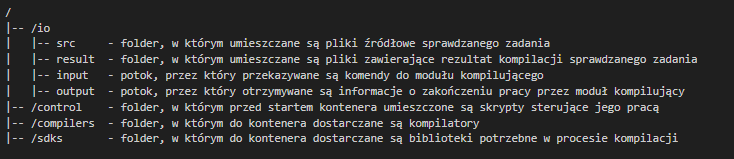
\includegraphics{img/3/orkiestrator-kontenerow-struktura-katalogow.png}
		}
		\caption{Struktura katalogów tworzona przy inicjalizacji modułu kompilującego. Źródło własne.}
		\label{fig:scheduler-directory-structure}
	\end{center}
\end{figure}
Ostatnim elementem inicjalizacji jest uruchomienie kontenerów poleceniem \textit{docker run} z obrazem \textit{wine-vs-runner} pozyskanym z obecnie funkcjonującego systemu STOS-WEB z argumentami:
\begin{itemize}
    \item \textit{--mount} -- powiązanie ścieżek systemu macierzystego z ścieżkami kontenera,
    \item \textit{--memory} -- ograniczenie zasobów pamięci RAM wykorzystywanej przez kontener,
    \item \textit{--cpus} -- ograniczenie zasobów procesora wykorzystywanych przez kontener,
    \item \textit{-d} -- uruchomienie kontenera bez blokowania terminala z kórego jest uruchamiany (\textit{detached}),
    \item \textit{--user} -- określenie użytkownika i~uprawnień kontenera.
\end{itemize}
oraz dodanie powiązanych z nimi obiektów do kolejki reprezentującej kontenery oczekujące na zlecenie zadania do sprawdzenia.

\subsubsection{Komunikacja z zarządcą}
Komunikacja z komponentem zarządcy odbywa się za pomocą wołań zwrotnych. Gdy zarządca otrzyma nowe zadanie, wywołuje metodę \textit{register\_new\_task} orkiestratora kontenerów, przekazując jej obiekt „TaskData” reprezentujący zadanie przesłane do sprawdzenia. Implementacja tej metody dodaje do kolejki obiekt przekazany w~argumencie. Komunikacja w~drugą stronę również odbywa się poprzez wołania zwrotne. Orkiestrator kontenerów udostępnia w~interfejsie metodę \textit{register\_task\_completion\_callback}, której argumentem jest funkcja przyjmująca obiekt sprawdzonego zadania oraz ścieżkę na dysku do plików rezultatu, której implementacja zapisuje w~liście przekazaną funkcję. Wszystkie funkcje z listy są wywoływane po sprawdzeniu zadania. Podejście to niesie za sobą korzyść zmniejszenia powiązania komponentów systemu. Umożliwia również, aby na zdarzenie sprawdzenia zadania nasłuchiwało wiele komponentów, mogą to być na przykład systemy logów, systemy tworzenia kopii zapasowych lub kilka instancji zarządców. Sprawia to, że system jest bardziej otwarty na rozbudowę o~nowe komponenty i~skalowanie.

\subsubsection{Przepływ zdarzeń orkiestratora kontenerów}
Orkiestrator kontenerów pozbawiony jest nieskończonej pętli aktywnie monitorującej stan i~wykonującj instrukcje. Zamiast tego jest sterowany zdarzeniami (rynsunek \ref{fig:scheduler-activity-diagram}), główna funkcja -- \textit{manage\_workers}, odpowiadająca za logikę biznesową wywoływana jest wtedy, gdy zmienia się stan kolejek zadań i~kontenerów. Implementacja metody sprawdza, czy w~zarówno w~kolejce zadań i~kolejce kontenerów znajdują się elementy, jeśli tak, pobiera po jednym elemencie i~rozpoczyna przetwarzanie zadania.

\begin{figure}[!ht]
	\begin{center}
		\resizebox{1\textwidth}{!} {
			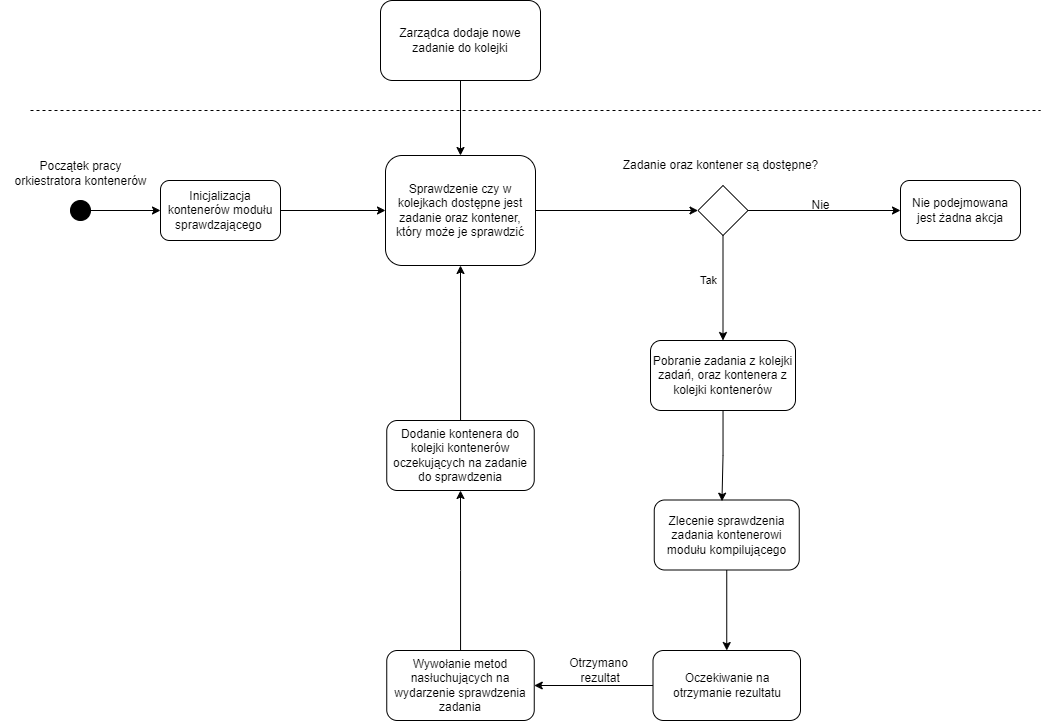
\includegraphics{img/3/orkiestrator-kontenerow-diagram-aktywnosci.png}
		}
		\caption[Diagram aktywności orkiestratora kontenerów]{Diagram wizualizujący przebieg pracy orkiestratora kontenerów. Źródło własne.}
		\label{fig:scheduler-activity-diagram}
	\end{center}
\end{figure}

Przetwarzanie zadania odbywa się wykonaniem metody \textit{process\_task}. Aby kontener modułu kompilującego mógł zacząć pracę, należy dostarczyć mu wszystkie pliki źródłowe przetwarzanego zadania skompresowane w~archiwum zip do katalogu \textit{io/src} katalogu współdzielonego. Archiwum tworzone jest modułem zipfile\cite{pythonZipfile}, zawierającym narzędzia do odczytu i~zapisu plików zip. Gdy archiwum znajduje się w~folderze, następuje wydanie polecenia do kontenera, poprzez wpisanie do potoku \textit{io/input} katalogu współdzielonego. Dostępne polecenia to:
\begin{itemize}
    \item \textit{vc-debug} - kompilacja w~trybie debugowania, generowane są dodatkowe informacje o~kodzie, zmiennych, funkcjach,
    \item \textit{vc-opt} - kompilacja z optymalizacją, w~procesie kompilacji poprawiana jest wydajność kodu wynikowego, może obejmować pominięcie zbędnych operacji, zmnianę struktury kodu, zmniejszenie rozmiaru plików wykonywalnych,
    \item \textit{vc-both} - kompilacja z optymalizacją w~trybie debugowania - połączenie poleceń vc-debug i~vc-opt.
\end{itemize}
Wydanie polecenia rozpoczyna proces kompilacji wewnątrz kontenera. Informacja o~zakończeniu kompilacji przekazywana jest poprzez potok \textit{io/output}, a~rezultat umieszczany jest w~katalogu \textit{io/result}. Orkiestrator kontenerów otwiera potok i~zapisuje go do zmiennej metodą \textit{open}, której argumentem jest ścieżka do potoku, a~następnie oczekuje na pojawienie się w~nim informacji i~odczyt metodą \textit{read}, która oprócz potoku przyjmuje w~argumencie maksymalną ilość odczytanych bajtów. Obie metody pochodzą z modułu os\cite{pytohnOs}. Po otrzymaniu informacji zwrotnej od kontenera, rezultat jest kopiowany do tymczasowego folderu przechowującego wyniki zadań, a~orkiestrator wywołuje wszystkie funkcje nasłuchujące na zdarzenie sprawdzenia zadania, przekazując im obiekt zadania oraz ścieżkę do skopiowanego rezultatu.

\lstset{style=python}
\begin{lstlisting}[caption = {Implementacja metody odczytującej informacje z potoku.}]
    # Wait for worker result 
    def watch_output_pipe(self, task_data: TaskData, worker_id: str) -> None:
        path = f'./worker_{worker_id}/io/output'
        if not os.path.exists(path):
            self.__stos_logger.error(f"watch_output_pipe: Path {path} does not exist.")
            return
        output_pipe = os.open(path, os.O_RDONLY)
        self.__stos_logger.info(f"watch_output_pipe: Waiting for task: {task_data.task_id} result from worker: {worker_id}")
        data = os.read(output_pipe, 1024)
        self.__stos_logger.info(f"watch_output_pipe: Result: {data} for task: {task_data.task_id} from worker: {worker_id}")
        os.close(output_pipe)
\end{lstlisting}

\subsubsection{Współbieżne przetwarzanie zadań}
W celu umożliwienia sprawdzania kilku zadań jednocześnie, dzieje się to w~sposób współbieżny. Python udostępnia narzędzia do tworzenia współbieżnych programów w~module threading\cite{pythonThreading}, zawierający wysokopoziomowe metody do zarządzania wątkami. Utworzone w~ten sposób wątki nie są jednak wykonywane równolegle, czyli w~danym momencie czasu wykonywana jest tylko instrukcja pochodząca z kodu jednego wątku programu, ale pozwala na wykonywanie innych operacji w~czasie oczekiwania na pojawienie się rezultatu zadania sprawdzanego przez kontener modułu kompilującego. Dzieje się tak ze względu na implementację interpretera Python, zawierającego w~sobię globalną blokadę interpretera (\textit{Global Interpreter Lock}\cite{pythonGlobalInterpreterLock}) zapobiegającą takiemu zachowaniu. Upraszcza to proces zarządzania sekcjami krytycznymi, czyniąc wiele operacji bezpiecznymi z perspektywy wykonywania współbieżnego bez zastosowania dodatkowych mechanizmów bezpieczeństwa, jednak tym samym nie wykorzystuje w~pełni możliwości wielordzeniowych procesorów. Aby zrównoleglić wykonywane operacje, należy wyłączyć globalną blokadę interpretera, budując go z kodu źródłowego z włączoną opcją \textit{--disable-gil} lub skorzystać z modułu multiprocessing\cite{pythonMultiprocessing}, który tworzy osobne procesy systemowe. W~implementacji orkiestratora kontenerów zastosowano moduł threading wraz ze standardowymi ustawieniami globalnej blokady interpretera, ponieważ ten komponent nie wykonuje skomplikowanych i~czasochłonnych operacji, a~jedynie odpowiada za zarządzanie kontenerami i~przepływ danych między nimi a~resztą systemu, więc wykonywanie go równolegle nie przyniosłoby wymiernego przyspieszenia działania systemu -- to etap kompilacji, który odbywa się w~kontenerach, jest najbardziej czasochłonny i~to własnie ten etap został zrównoleglony dzięki przeprowadzaniu go w~wielu instancjach kontenerów.

Nowe wątki są tworzone w~implementacji metody \textit{manage\_workers}, która sprawdza, czy w~kolejkach znajdują się zadanie oraz kontener, który mógłby je przetworzyć, a~następnie tworzy nowy wątek odpowiedzialny za przetworzenie zadania. Mimo że pojedyncze operacje na kolejkach pochodzących z modułu queue\cite{pythonQueue} sa bezpieczne wielowątkowo, to w~metodzie występuje sekcja krytyczna składająca się z kolejnego sprawdzenia stanu i~pobrania elementów z kolejki. Aby zapobiec sytuacji, w~której wykonanie funkcji w~jednym wątku sprawdzi, że kolejki nie są puste i~wejdzie do bloku warunkowego, a~inny wątek w~tym czasie pobierze element z kolejki, zastosowano mechanizm semafora binarnego, uniemożliwiającego wielu wątkom jednoczesne wykonywanie kodu znajdującego się w~sekcji krytycznej.

\lstset{style=python}
\begin{lstlisting}[caption = {Implementacja metody rozpoczynającej przetwarzanie zadania.}]
    @override
    def manage_workers(self) -> None:
        with self.__lock:
            while not self.__workers_queue.empty() and not self.__tasks_queue.empty():
                task = self.__tasks_queue.get()
                workerId = self.__workers_queue.get()
                thread = threading.Thread(target=self.process_task, args=(task, workerId))
                thread.start()
\end{lstlisting}